\documentclass[Royal,times,sageh]{sagej}

\usepackage{moreverb,url,natbib, multirow, tabularx}
\usepackage[colorlinks,bookmarksopen,bookmarksnumbered,citecolor=red,urlcolor=red]{hyperref}



% tightlist command for lists without linebreak
\providecommand{\tightlist}{%
  \setlength{\itemsep}{0pt}\setlength{\parskip}{0pt}}



\usepackage{booktabs}
\usepackage{longtable}
\usepackage{array}
\usepackage{multirow}
\usepackage{wrapfig}
\usepackage{float}
\usepackage{colortbl}
\usepackage{pdflscape}
\usepackage{tabularx}
\usepackage{xltabular}
\usepackage{threeparttable}
\usepackage{threeparttablex}
\usepackage[normalem]{ulem}
\usepackage{makecell}
\usepackage{xcolor}


\begin{document}


\setcitestyle{aysep={,}}

\title{Intoducing CommuteCA: An open data package with datasets and
standardized methods for job accessibility analyses in Canada}

\runninghead{Anon1 \& Anon2.}

\author{Anon1\affilnum{}, Anon2\affilnum{}}

\affiliation{\affilnum{}{}}

\corrauth{Anon1 - Address.}

\email{\href{mailto:Anon1@anon.org}{\nolinkurl{Anon1@anon.org}}}

\begin{abstract}
The Canadian Census provides detailed information on the labour force
population and how they commute to work. However, the original Census
microdata files are confidential, and even when access is granted,
preparing the data for analysis is not straightforward. Based on this,
this paper introduces CommuteCA, an open data product in the form of an
R package, providing analysis-ready data and standardized methodologies
for conducting job accessibility analyses in Canada using data from the
2021 Census of Population. For metropolitan areas and urban
agglomerations, the package provides information on the labour force by
transportation mode and education level, as well as on the number of
jobs by occupation category, at the census tract level. In addition,
CommuteCA provides calibrated impedance functions for all municipalities
for four transportation modes (walking, cycling, public transit, and
car-motorized vehicles), as well as calibrated functions according to
education levels. The package also includes standardized methodologies
in the form of R Markdown templates for conducting accessibility
analyses using either the Census microdata files or the processed
datasets, as well as customized functions that facilitate users'
analyses.
\end{abstract}

\keywords{opportunity; employment; impedance; travel; transport;}

\maketitle

\section{Introduction}\label{introduction}

The objective of this paper is to present \{CommuteCA\}, an Open Data
Product (ODP) containing analysis-ready data from the 2021 Census of
Population of Canada \citep{statisticscanada2023}, along with
standardized methodologies for performing urban accessibility analyses.
ODPs result from open and transparent processes that transform raw data
to make them ready for analysis \citep{arribas-bel2021}. Unlike open
data in general, ODPs are characterized mainly by the added value they
provide to raw data, but also by their enhanced usability and ease of
access.

\{CommuteCA\} provides analysis-ready data and standardized
methodologies for accessibility analyses in any study area in Canada.
The source of these data is the restricted and confidential microdata
files of the 2021 Census of Population \citep{statisticscanada2023},
managed by Statistics Canada. Census data have proved valuable in
investigations of urban accessibility, defined as the ease of reaching
spatially distributed opportunities \citep{hansen1959}, whether by
providing land use tables containing the locations of populations and
opportunities
\citep{merlin2017, jassochávez2025, cui2020, delmelle2021}, or by
linking accessibility indicators with individual outcomes, such as their
impact on employability levels
\citep{bastiaanssen2025, bastiaanssen2021}, job informality
\citep{boisjoly2017, duarte2023}, and job commuting distance
\citep{hu2017}.

To create \{CommuteCA\}, we extracted and processed all the data needed
to create land use tables, in which, for each Canadian census tract, we
counted the number of people in the labour force; the number of people
who commute to work by walking, cycling, public transportation, and by
car, van, motorcycle, or other automotive vehicles; and the number of
employment opportunities. We also provide additional land use tables
with the workforce and job opportunities classified by education level,
for accessibility analyses that aim to consider a potential match
between population scholarly attainment and job position requirements.
In addition, we retrieved respondents' commuting durations and
calibrated impedance functions, categorized by transportation mode
and/or education level, for each Census Division (municipality), Census
Metropolitan Area or Census Agglomeration, and Canadian province in
order to represent the commuting behaviour of the Canadian population.
We also created \texttt{R} Markdown templates demonstrating how to
conduct accessibility analyses for any study area within Canada,
providing standardized methodologies ranging from the very basics of
programming in \texttt{R} to calculating accessibility models and
accessibility maps to inform transportation planning and policy.

Although Statistics Canada offers Public Use Microdata Files and
documentation for the 2021 Census of Population \citep{PUMFCensus2021},
these files do not include geographic references below the municipal
(Census Division) level, nor do they contain the workplace location of
employed respondents. In addition, the original census microdata files
are confidential and require access to Research Data Centres (RDC),
Statistics Canada offices, following a lengthy approval process, which
makes it difficult for urban planners and transportation researchers to
make data-driven decisions. Even when access is granted, preparing the
data for analysis is not straightforward, given its size and complexity.
Moreover, the process of extracting information of interest from surveys
like the Census is time-consuming, technically challenging, and prone to
error, particularly for analysts without extensive experience working
with these files.

Despite the valuable advances achieved by other packages, especially
\{cancensus\} \citep{cancensus}, which has provided analysis-ready data
frames and spatial data in multiple formats, as well as convenience
functions for working with Canadian census data, these packages do not
fully support urban accessibility analyses. To our knowledge, no
existing package has yet released the data and standardized methodology
required to support urban accessibility analyses for any study area in
Canada. In particular, existing packages do not provide workplace
locations at the intra-urban level or impedance functions that represent
population travel behaviour when commuting to work, nor do they provide
a standardized methodology for conducting accessibility analyses.

More than ever, accessibility analyses are sparking the interest of
planning practitioners in Canada (e.g., \citet{nicknewstead2024}).
Therefore, reducing barriers to accessing and using rich but
difficult-to-access and complex datasets, such as the Canadian census,
is a valuable effort that can contribute to more data-driven
decision-making in urban planning.

\{CommuteCA\} is part of a broader research effort to implement and
inspire the best principles of open spatial science
\citep{paez_open_2021, brunsdon_opening_2021}. As part of this effort,
we aim to create ODPs from datasets that, in our perspective, could be
more widely used by transportation planners and scholars because they
contain valuable variables and for provide high-quality data, often at
the national level. We released \{CommuteCA\} as an \texttt{R} package
containing code, data, and documentation in a standardized format that
can be installed and used by \texttt{R} users, providing an effective
medium for distributing analysis-ready data. This approach has also been
demonstrated by other ODPs \citep{dossantos2025, soukhov2023} and
analyses based on them \citep{dossantos2026, soukhov2023a}.

In the following sections, this paper discusses the 2021 Census of
Population, our main data source, and the process implemented to
retrieve and organize into an ODP. Next, we a case study using the
datasets and methodological framework to assess the accessibility to
employments in the City of Toronto, in order to spark the interest of
potential users. This ODP provides not only data and easy-to-use
\texttt{R} Markdown templates, but also all the code and documentation
that make this research project completely reproducible.

\section{Canadian Census}\label{canadian-census}

The most recently released Census in Canada was held in 2021, collecting
information on the Canadian population to support planning in diverse
areas, including public transportation and skills training to improve
employment outcomes \citep{statisticscanada2023}. The microdata file for
the 2021 Canadian Census contains almost 9 million observations and
includes almost 900 variables. The data are hierarchically organized
into five units of statistical analysis: persons, census families,
economic families, households, and dwellings. Each record in the
microdata file represents an individual response, which is later grouped
into the higher hierarchy levels.

The 2021 Census was Canada's 23rd national census and showed that the
Canadian population increased by 5.2\% relative to the previous census,
reaching almost 37 million people. The majority (75\%) of households
received a short-form questionnaire covering topics related to language,
sex at birth, gender, marital status, and age, while the remaining 25\%
received a long-form questionnaire that also covered topics related to
activities of daily living, socio-cultural information, mobility,
education, and labour market activity. The census data are accompanied
by reference guides designed to help users better understand the files.
Among these reference guides, the Commuting Reference Guide
\citep{DictCensus2021}, along with the Labour Force Reference Guide,
contains the variables most relevant for transportation analyses.

\subsection{Commute, Labour Force, and Education Reference
Guides}\label{commute-labour-force-and-education-reference-guides}

The long-form 2021 Canadian Census contains questions related to the
Canadian labour force and commuting to work \citep{DictCensus2021}. The
labour force consists of people aged 15 years and over living in private
households who are either employed or unemployed but actively looking
for work. In the labour section, respondents answered questions related
to employment status, the number of hours and weeks worked in the
previous year, the main reasons for not working the full year (when
applicable), and more. Employed respondents were also asked questions
related to their industry sector, occupation, employment status
(part-time or full-time), and more. Unemployed respondents were asked
about the main reason for being unable to find work, the reason for not
accepting a new job (when applicable), and whether they planned to start
a new job (when applicable).

In the section related to commuting, the questions referred to the
journey to work. These questions include whether respondents worked at
home (including farms), outside Canada, or had a fixed workplace
address. Other questions include the workplace location, main mode of
commuting, other commuting modes, vehicle occupancy, commuting duration,
and departure time.

According to the 2021 Canadian Census, about 30.3 million Canadians were
aged 15 years or older and living in private households, making them
eligible to participate in the labour force (about 82\% of the
population). However, the labour force participation rate was 63.7\%
(about 19.3 million people), meaning that approximately 11 million
people were unemployed but were not actively seeking work due to early
retirement, education, family care responsibilities, illness or
disability, personal choice, or because they were discouraged workers -
cases in which a person wanted a job but stopped looking because they
believed no work was available or could not find suitable employment in
their local labour market. Among those in the labour force, the
unemployment rate was about 10.3\%. The 2021 Census revealed that the
labour market was still being affected by the COVID-19 pandemic, with
the number of people in the labour force showing a slight decline, from
19.5 million in 2016 to 19.3 million.

The number of employed people was approximately 17.3 million. Of that
total, 4.2 million worked from home, representing 24.3\% of the employed
workforce - a share three times higher than the proportion observed in
2016. The 2021 Census also revealed that approximately 13 million people
commuted to work. Among them, the majority (84\%) commuted by car,
truck, or van; 8\% used public transportation; 5\% walked; and 1\%
cycled. In terms of commuting duration, 32\% of commuters travelled for
less than 15 minutes, 35\% between 15 to 29 minutes, 19\% between 30 to
44 minutes, 7\% for 45 to 59 minutes, and 7\% for 60 minutes or more.
For Canadians aged 15 years and over, 16\% do not have a certificate,
diploma, or degree, while 27\% have a high school diploma or equivalency
certificate as their highest level of education, and 57\% have earned at
least a postsecondary certificate.

\section{Data process}\label{data-process}

Figure \ref{fig:process-figure} presents a diagram illustrating the
processes applied to the Census microdata files to create the
\{CommuteCA\} datasets. These datasets were created with the intention
of providing all the data required to calculate job accessibility for
any study area in Canada.

\begin{figure}

{\centering 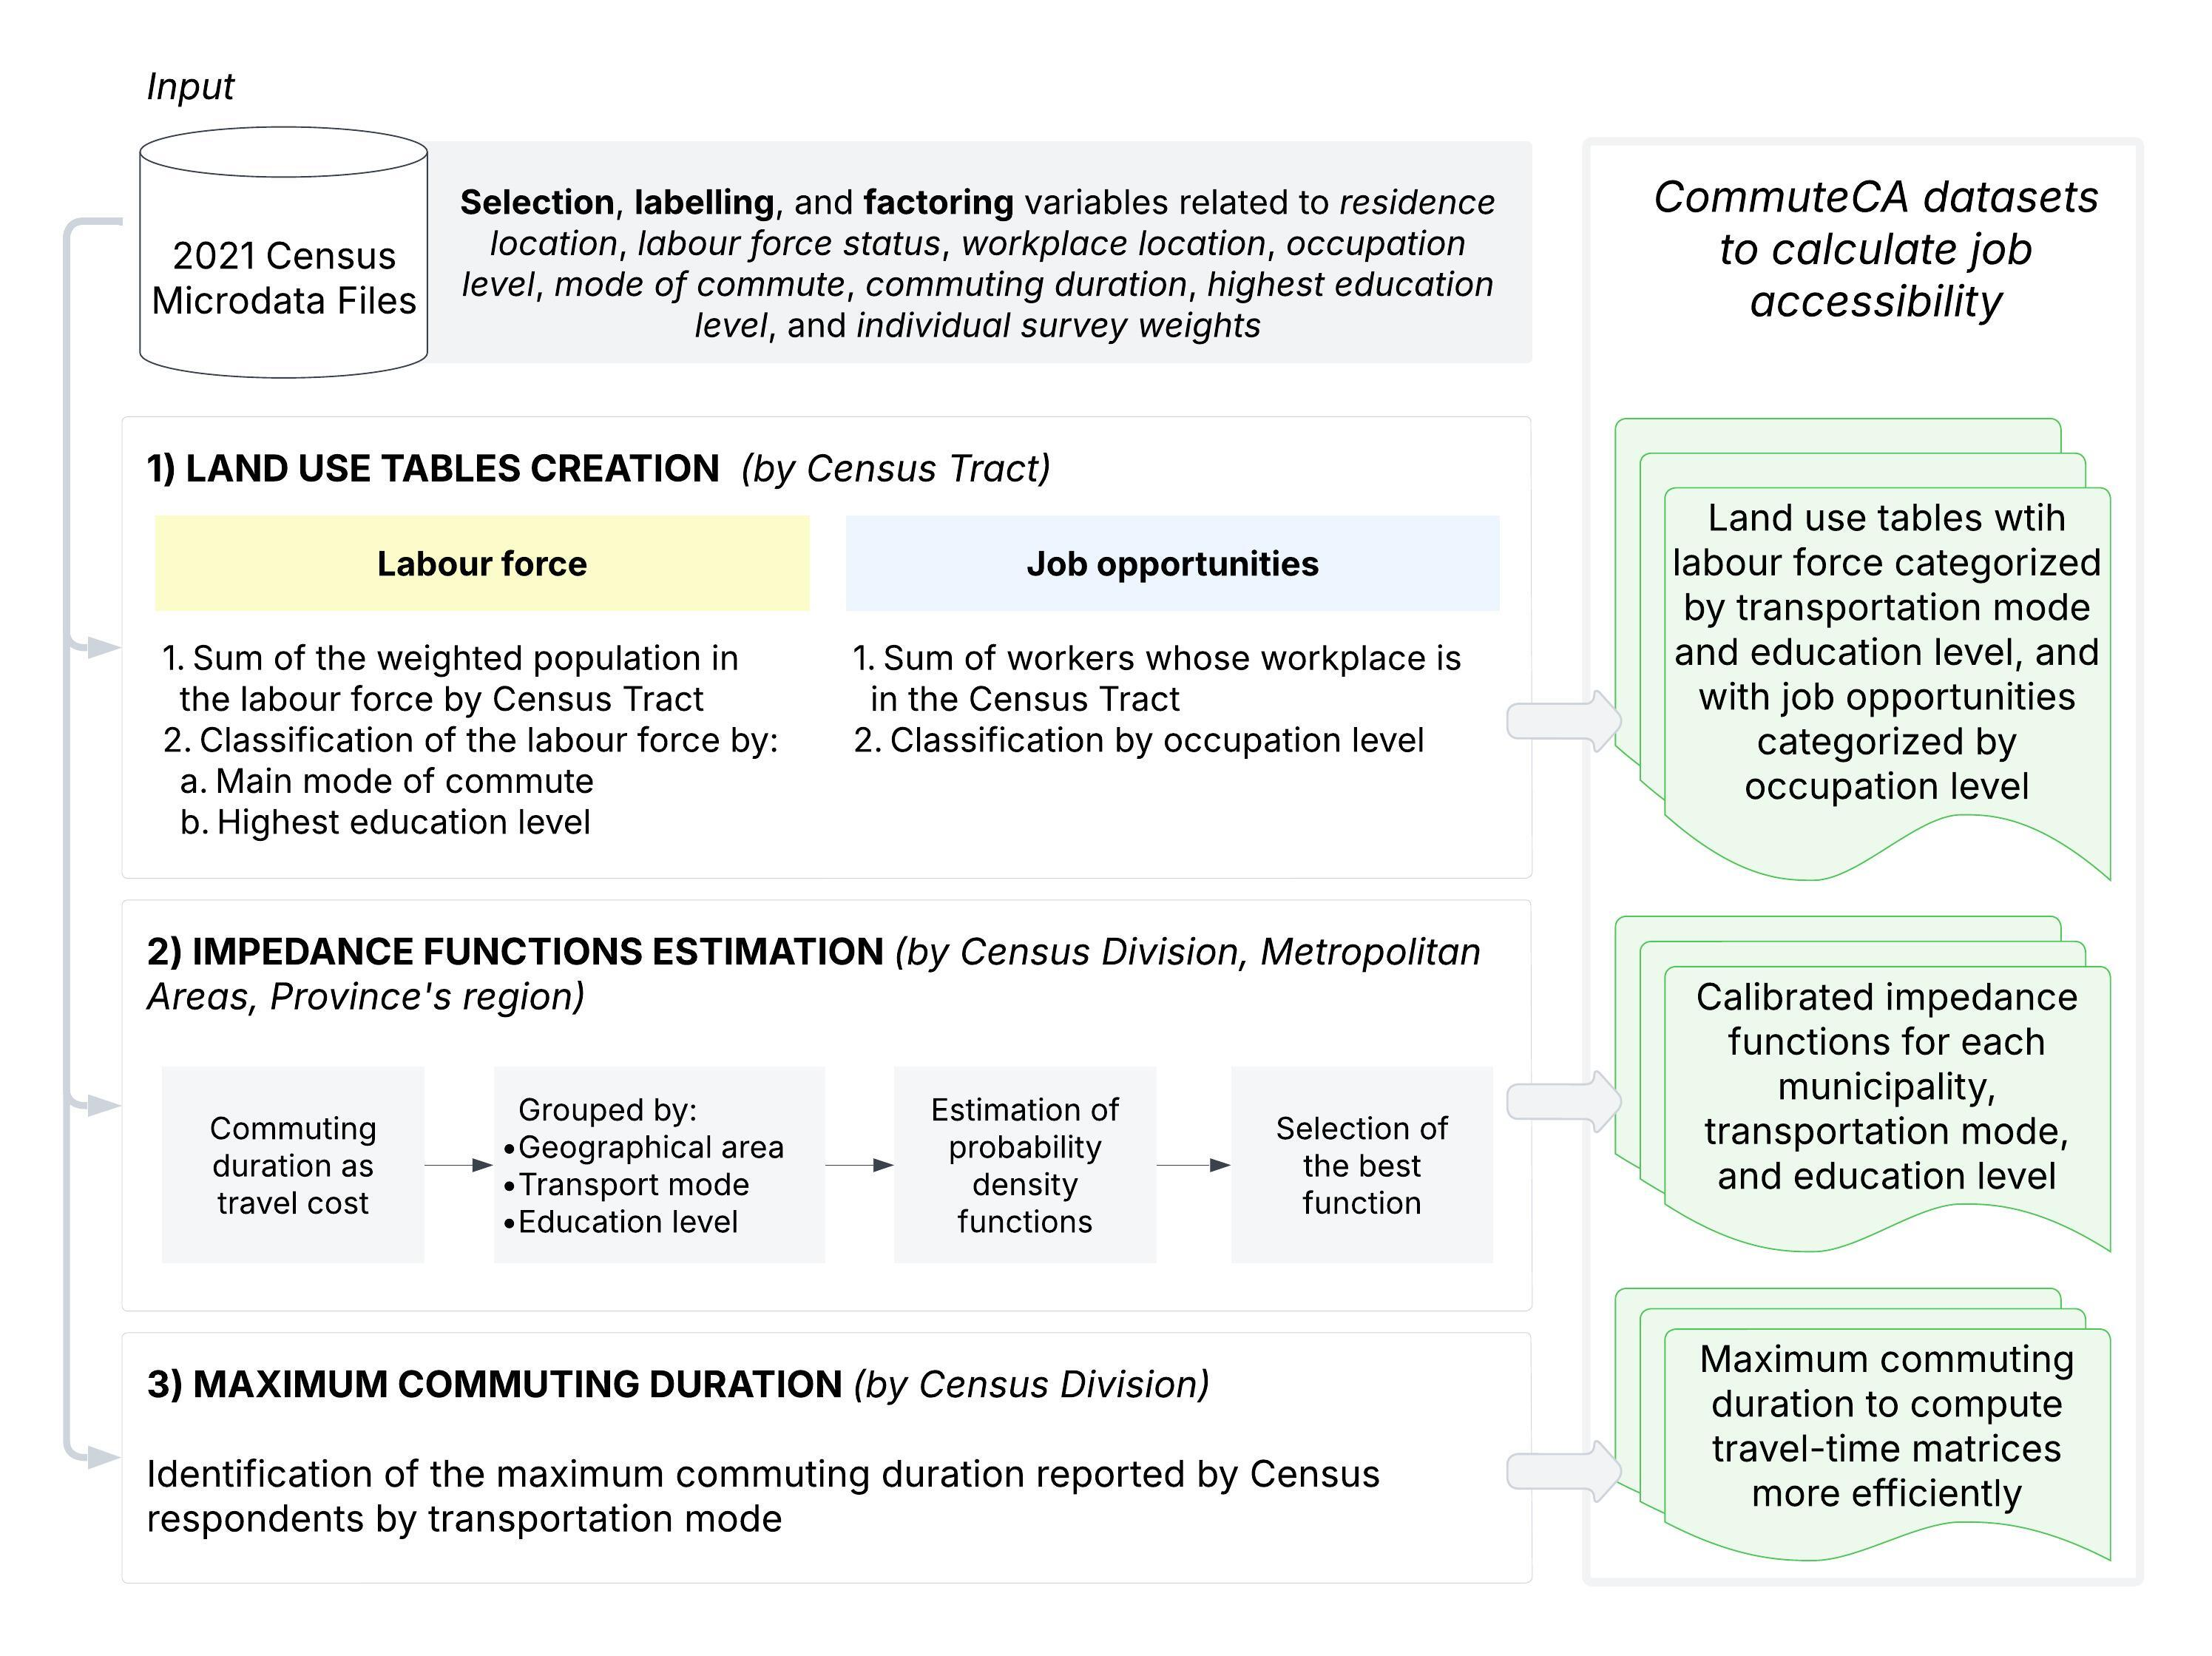
\includegraphics[width=1\linewidth]{CommuteCA_datasets} 

}

\caption{CommuteCA datasets obtained from the 2021 Canadian Census microdata files.}\label{fig:process-figure}
\end{figure}

Acessibility refers to the ease of reaching spatially distributed
opportunities \citep{hansen1959} and results from the interaction
between land use and transportation systems \citep{geurs2004}. Based on
this, we grouped the inputs required for these calculations into three
categories: 1) a land use table reporting, for each spatial unit, the
number of opportunities - in this case, employment opportunities -, and
the number of people competing for these opportunities when competition
is considered by the accessibility measure; 2) a routing table
containing the travel costs between each origin and destination,
typically expressed as travel-time matrices for one or more
transportation modes; and, 3) one or more impedance functions
representing the difficulty of accessing opportunities. \{CommuteCA\}
provides the first and third of these components, while also proving
inputs to generate the second using routing engines such as \{r5r\}
\citep{pereira2021}.

We begin by creating land use tables for all areas containing a Census
Tract (CT). CTs are intra-municipal spatial units with populations
ranging from 2,500 to 7,500 people, with an average of 5,000, and are
located in Census Metropolitan Areas (CMAs) and Census Agglomerations
(CAs) that had a population greater than 50,000 at the previous census
(2016). Although CTs do not cover the entire country, 84\% of the
Canadian population lived in a CMA or CA (over 31 million people). CTs
are distributed across all Canadian provinces, except Prince Edward
Island, whose total population was only slightly more than 154,000 in
2016.

In terms of the labour force, \{CommuteCA\} contains land use tables
with data on the total labour force in each CT, as well as the labour
force classified by highest education level and/or transportation mode.
First, we summed the weighted population within the labour force in each
CT. Then, we identified the main transportation mode used to commute to
work, when applicable, and classified it into four categories:
``Car/Motorized'' (car, truck, van, or motorcycle), ``Public Transit''
(bus, subway, rail, streetcar, train, or passenger ferry), ``Walk'', and
``Bike''. For workers who worked remotely or did not have a fixed
workplace, as well as unemployed people, we used the category ``Other or
non-commuter''. Next, we classified members of the labour force based on
their highest education level into three categories: ``High school or no
certificate'', ``College or apprenticeship certificate'' to represent
postsecondary certificate or diploma below university level, and
``University certificate or higher''.

For job opportunities, we summed the number of workers whose reported
workplace was located in each CT and used this total as an estimate of
the number of employment opportunities within the CT. We also classified
these job opportunities according to the 2021 National Occupational
Classification (NOC) and its Training, Education, Experience and
Responsibilities (TEER) categories. As a result, the tables provide
estimates of the number of ``Management and professional'' jobs,
corresponding to management and professional occupations that generally
require completion of a university degree or previous experience and
expertise in subject-matter knowledge from a related occupation (TEER 0
and 1); ``College or apprenticeship'', referring to occupations in TEER
2 and TEER 3, which usually require completion of a postsecondary
education program or apprenticeship training program; and ``High school
or short-term experience'', referring to occupations that usually
require completion of secondary school or a short work demonstration,
with no formal educational requirements.

When generating travel-time matrices using routing engines such as
\{r5r\}, analysts must specify a maximum trip duration - that is, the
longest travel time (in minutes) considered during route calculation -
to avoid unnecessary computations. For each Census Division
(municipality), regardless of whether it is located within a CMA or CA,
we identified the maximum commuting duration reported by Census
respondents.

Next, we estimated the best impedance functions to represent the
commuting behaviour of Canadians. We adopted Probability Density
Functions (PDFs) in which an impedance function can be interpreted as
the probability density of a trip occurring for each value of travel
cost duration, following the approach of \citet{soukhov2024},
\citet{sveda2023}, and \citet{dossantos2026}. We applied the
\{fitdistrplus\} package \citep{delignette2015fitdistrplus} to calculate
the best-fitting PDF for every Census Division (municipality), CMA, and
Province, transportation mode (walking, cycling, public transit, and
car/motorized) and/or education level, by modelling commuting duration
as travel cost and testing uniform, negative exponential, gamma, normal,
and lognormal distributions. Then, we selected the best impedance
function based on the lowest Akaike Information Criterion value
\citep{akaike1974}.

In addition to these datasets that enable calculating job accessibility
for CMAs or CAs in Canada, we also created testing datasets based on the
2021 Census of Population. These testing datasets were synthetically
generated and contain variables for accessibility analyses to make it
possible for analysts to practice coding outside Statistics Canada
offices or RDCs, since the access to the census microdata files is
restricted. One of these datasets has 250,000 observations distributed
across Canada and contains 17 variables, such as respondent identifiers
and sample weight, geographical information, status in the labour force,
and commuting to work variables. The second dataset represents
respondents living in the City of Toronto, contains over 50,000
observations and 32 variables, that in addition to the previous set of
variables, also includes sociodemographic variables that can be used to
test regression models, such as income, race, and gender.

All code used to generate the \{CommuteCA\} datasets is publicly
available through the project's GitHub repository, allowing researchers
to reproduce the datasets, verify the implementation, identify and
correct potential errors, and adapt the workflows to their own
applications.

\subsection{Research data centre vetting
process}\label{research-data-centre-vetting-process}

All datasets included in \{CommuteCA\} were subjected to the
confidentiality rules for the 2021 Census of Population through a
vetting process conducted at the RDC. To be released, \{CommuteCA\}
datasets had to comply with rules related mainly to minimum geographic
area sizes, statistical outputs, and counts. According to the vetting
rules, statistics must not be released for identifiable geographic areas
containing fewer than a minimum number of persons. For place-of-work
data, which are the source of the data used to produce all our datasets,
the population under consideration is the employed labour force.

In addition, all statistics other than counts must be based on weighted
data and must be calculated from at least a minimum number of
respondents whose combined weights must also exceed a minimum threshold
to be releasable. These statistics must also follow a specified rounding
system that varies according to sample size. For counts, all values must
be weighted and rounded to the nearest multiple of five.

\section{Standardized methodologies and
fuctions}\label{standardized-methodologies-and-fuctions}

Having provided the datasets required to calculate accessibility models,
\{CommuteCA\} also provides a collection of \texttt{R} Markdown
templates containing the code (including personalized functions) needed
to estimate these models and assess the relationship between
accessibility and employment outcomes. Therefore, the package provides a
transparent and standardized methodology for conducting transportation
analyses using the 2021 Canadian Census.

Figure \ref{fig:templates-figure} presents a diagram illustrating the R
Markdown templates available in \{CommuteCA\}. As shown in the figure,
these templates enable analysts to estimate accessibility models at the
CT level for multiple CMAs and CAs without requiring special access to
the census microdata files. In addition, they allow analysts to model
job accessibility for any study area in Canada, including areas outside
metropolitan areas, at the Dissemination Area (DA) level - a spatial
unit smaller than the CT, with a population between 400 and 700 people,
which was not included in the package datasets because of the
confidentiality restrictions defined by Statistics Canada.

\begin{figure}

{\centering 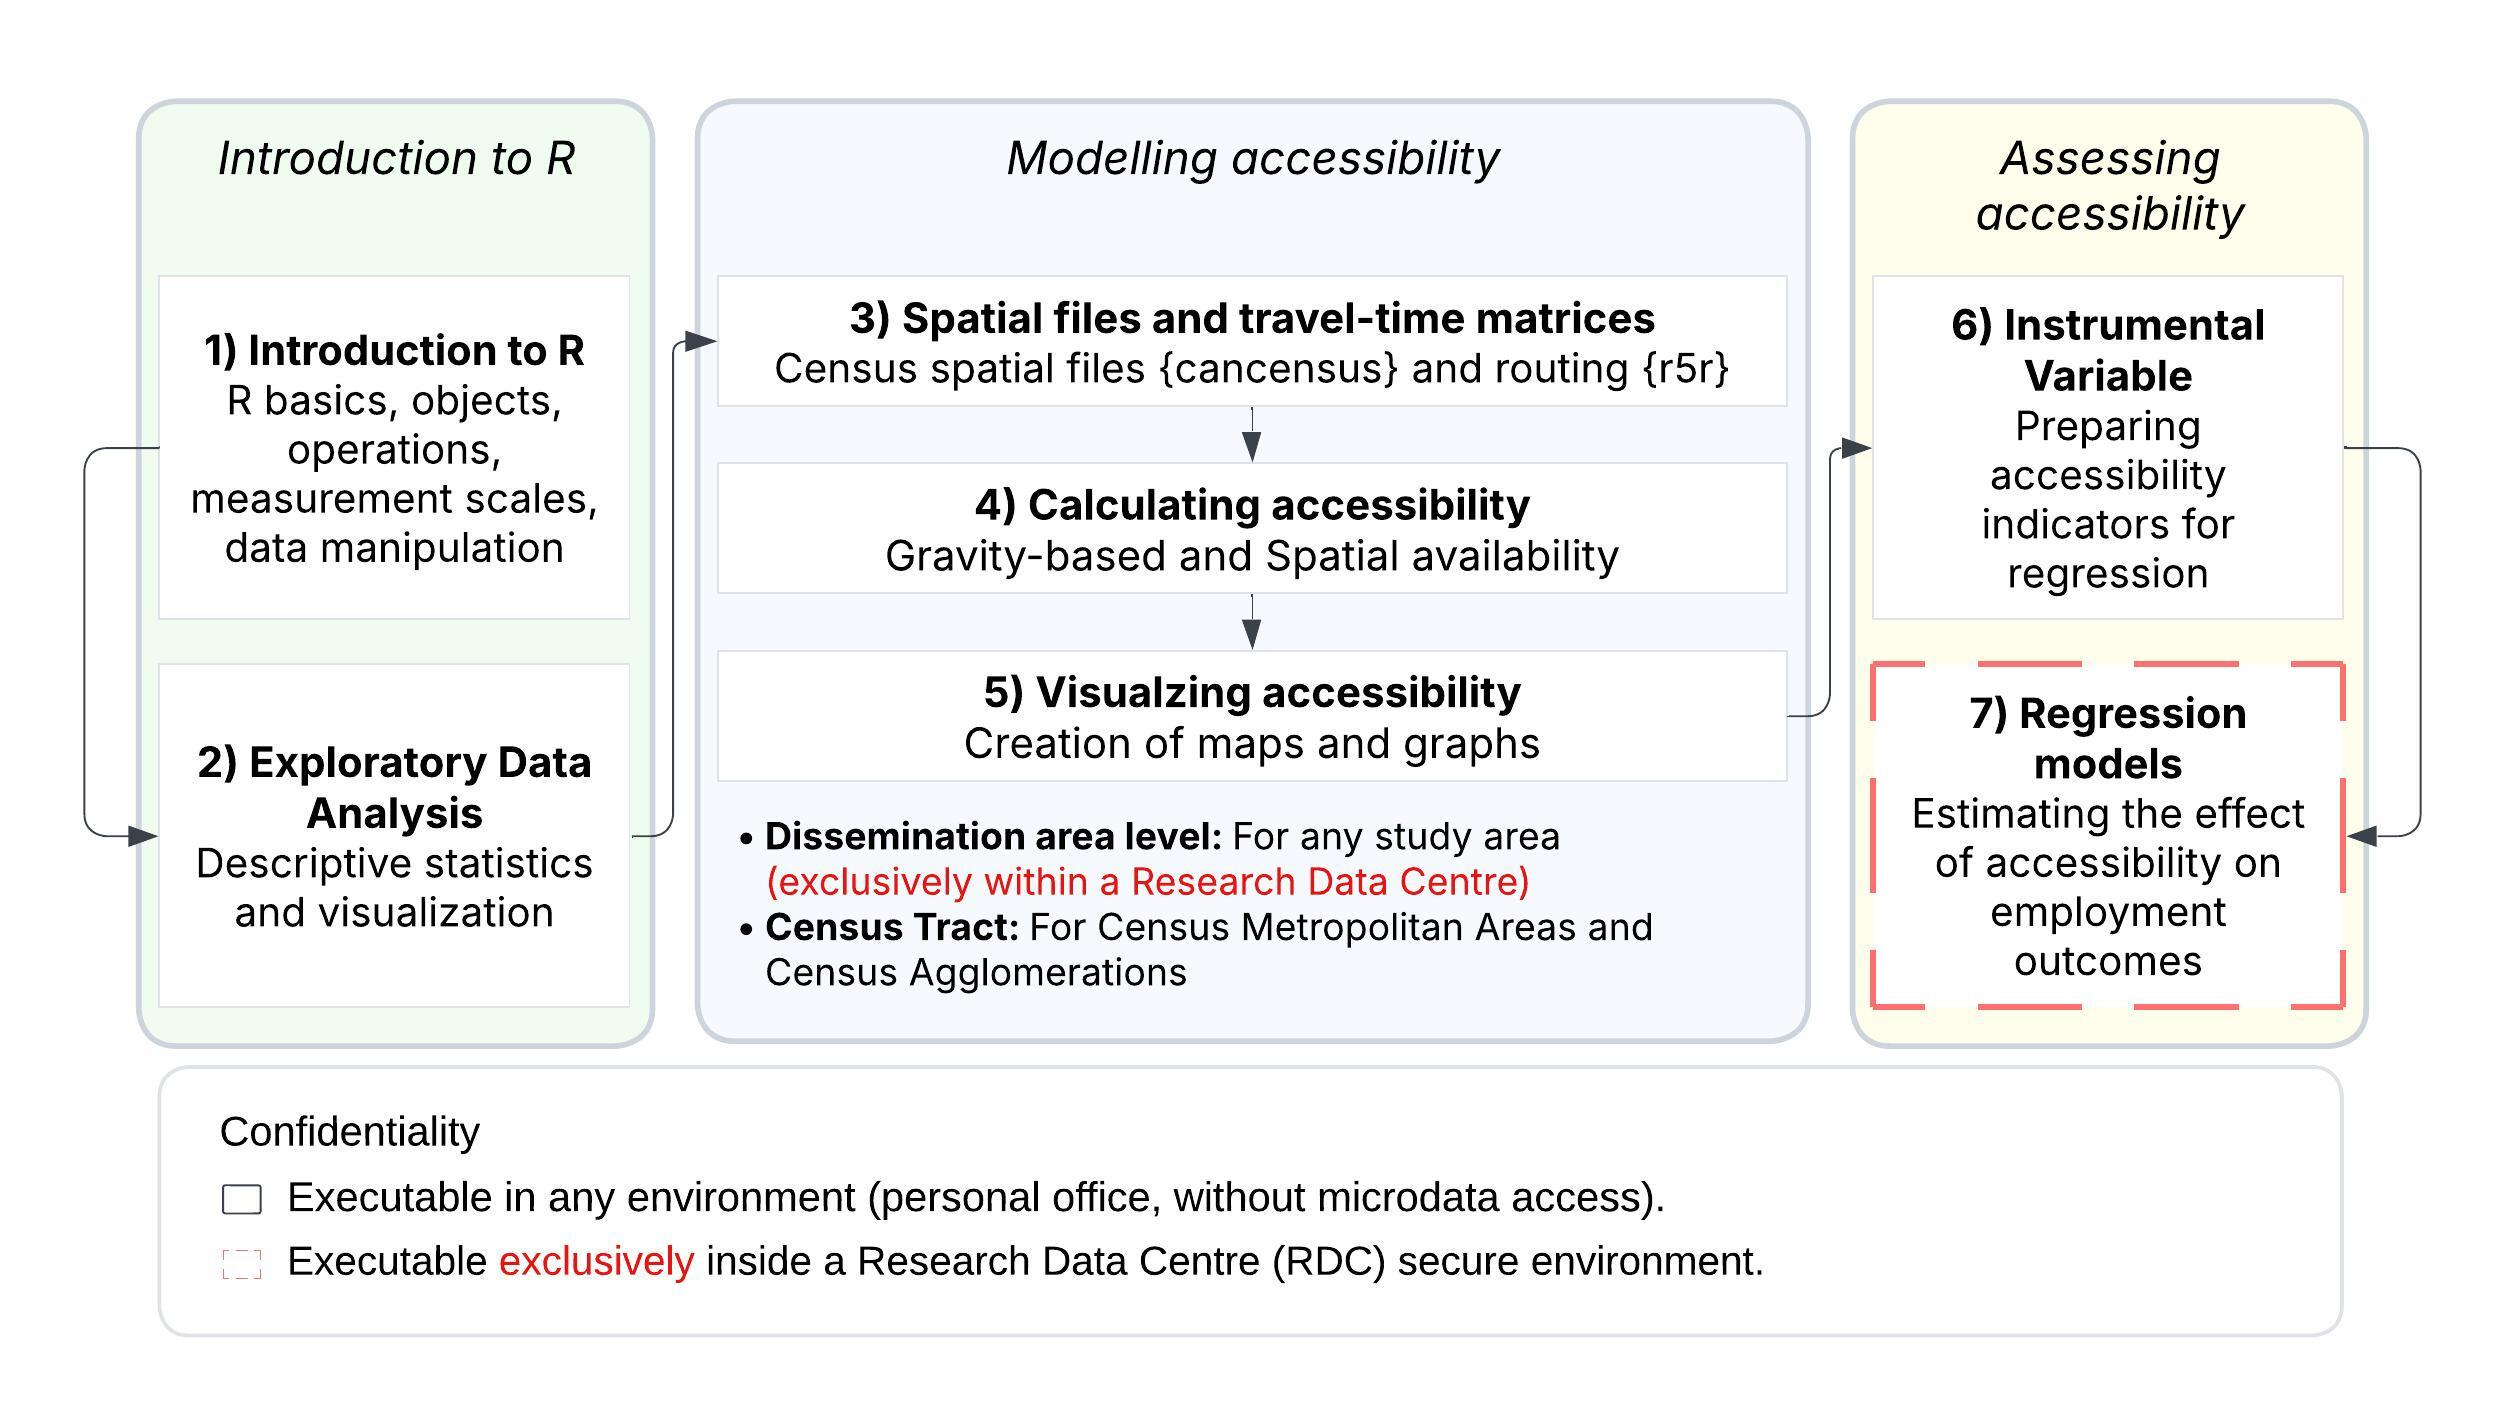
\includegraphics[width=1\linewidth]{CommuteCA_rmarkdown_template} 

}

\caption{R Markdown templates available in CommuteCA to perfom accessibility analyses.}\label{fig:templates-figure}
\end{figure}

In total, \{CommuteCA\} contains a couple of \texttt{R} Markdown
templates that guide analysts through an accessibility analysis, from an
introduction to \texttt{R} to the identification of accessibility
thresholds. They are divided into three groups: Introduction to
\texttt{R} (Templates 1 and 2), Accessibility Modelling (Templates 3 to
5), and Assessing Accessibility (Templates 6 to 7). The first template
provides an introduction to the \texttt{R} language. It also introduces
literate programming, data objects, basic operations, data measurement
scales, and data manipulation techniques in \texttt{R}. The second
template introduces Exploratory Data Analysis (EDA), demonstrating how
to produce descriptive statistics and create appropriate visualizations
for different data types.

The accessibility modelling templates begin with the third template,
which guides analysts in organizing census spatial data and demonstrates
how to obtain census spatial files using the \{cancensus\} package and
how to generate travel-time matrices using the \{r5r\} routing engine.
The forth template explains how to calculate job accessibility using the
traditional Hansen accessibility measure (gravity model) and the spatial
availability model proposed by \citet{soukhov2023a}. The fifth template
explains how to plot maps to visualize job accessibility.

The remaining templates focus on assessing accessibility outcomes using
the accessibility models generated in the previous stage. The sixth
template demonstrates how to create spatial filters for accessibility
indicators so that they can be incorporated into regression models
estimating the effects of accessibility on the probability of employment
and labour force participation. Finally, the seventh template
demonstrates how to estimate these regression models, including the
processing of socioeconomic, demographic, and environmental variables.

The package also includes customized functions that allow users to
select the best impedance function for a study area, plot theoretical
impedance values, calculate accessibility indicators, and create spatial
filters for the accessibility indicators.

\section{Results}\label{results}

\subsection{\{CommuteCA\} data sets}\label{commuteca-data-sets}

\{CommuteCA\} contains labour force and job opportunity estimates for
6,002 CTs, representing 96\% of the 6,247 CTs in Canada. Almost 14.7
million people in the labour force are represented in the included CTs,
representing around 77\% of the Canadian labour force. The labour force
not included in the dataset is composed of people who do not live in
metropolitan areas or who live in CTs excluded during the Statistics
Canada vetting process. Around 53\% of the labour force commuted by
car-motorized modes, followed by 6.5\% who commuted by public
transportation. Active commuters (walking or cycling) represented less
than 4\% of the labour force, while commuters who used non-specified
modes and non-commuters, due to being unemployed or because they were
working from home, represented 37\% of the labour force. Due to this
high share of the labour force not commuting to work, aggravated by the
COVID-19 pandemic, we also made available datasets with the non-commuter
labour force distributed across the other transportation modes,
according to the share of these modes in each CT. In terms of education,
the majority of the labour force had a certificate or degree above high
school, with 40\% having a university certificate or higher and around
28\% having a college or apprenticeship certificate.

Almost 70\% of the job opportunities in Canada are represented in the
\{CommuteCA\} datasets (around 11.8 million). Again, the jobs not
included in the dataset are either located in CTs excluded during the
vetting process or outside metropolitan areas. According to the TEER
categories, around 38\% of these job opportunities are categorized as
management or professional positions, which are usually occupied by
workers with at least a university degree or certificate; around 35\%
refer to positions that require college or apprentice certificates, and
the remaining 27\% are positions for which no certification or only a
high-school certification is required.

In most cases (80\%), the municipalities have impedance functions for
all four transportation modes. In some cases, the package does not
include an impedance function because there were no minimal labour force
respondents who reported commuting using a given mode in the sample. For
almost 15\% of the municipalities, only three impedance functions were
provided, while for less than 6\% only two functions were provided. We
were able to estimate impedance functions for car/motorized travel and
walking in all municipalities, while functions for public transit and
cycling were estimated for 90\% and 84\% of municipalities,
respectively.

\{CommuteCA\} contains maximum travel times and impedance functions for
all 293 Census Divisions in Canada. The maximum travel time identified
was 240 minutes (4 hours) for all four transportation modes:
car/motorized, public transit, walking, and cycling. The shortest
maximum travel time identified was 5 minutes for cycling in Les
Etchemins, Quebec. For the other modes, the shortest maximum travel
times were 15 minutes for walking (identified in Guysborough, Nova
Scotia), 30 minutes for public transit (identified in Communauté
maritime des Îles-de-la-Madeleine, Quebec), and 90 minutes for
car/motorized travel (identified in Kitikmeot, Nunavut).

\subsection{Case study}\label{case-study}

This section presents an application of the \{CommuteCA\} \texttt{R}
package using a selected study area. The application demonstrated in
this case study can be conducted by any user who installs the package,
without requiring access to the restricted microdata files of the 2021
Canadian Census. Installation instructions and examples of applications
of the \{CommuteCA\} \texttt{R} package are available in the vignettes
in the project's GitHub repository, and all analyses presented in this
section were conducted using the \texttt{R} Markdown templates provided
with the package.

For this demonstration, we will realize a multimodal accessibility
analysis for the City of Toronto, in Ontario, Canada (Figure
\ref{fig:study-area-map}). According to the 2021 Canadian Census
\citep{statisticscanada2023}, almost 2.8 million residents live in this
area, which covers approximately 631 square kilometres.

\begin{figure}
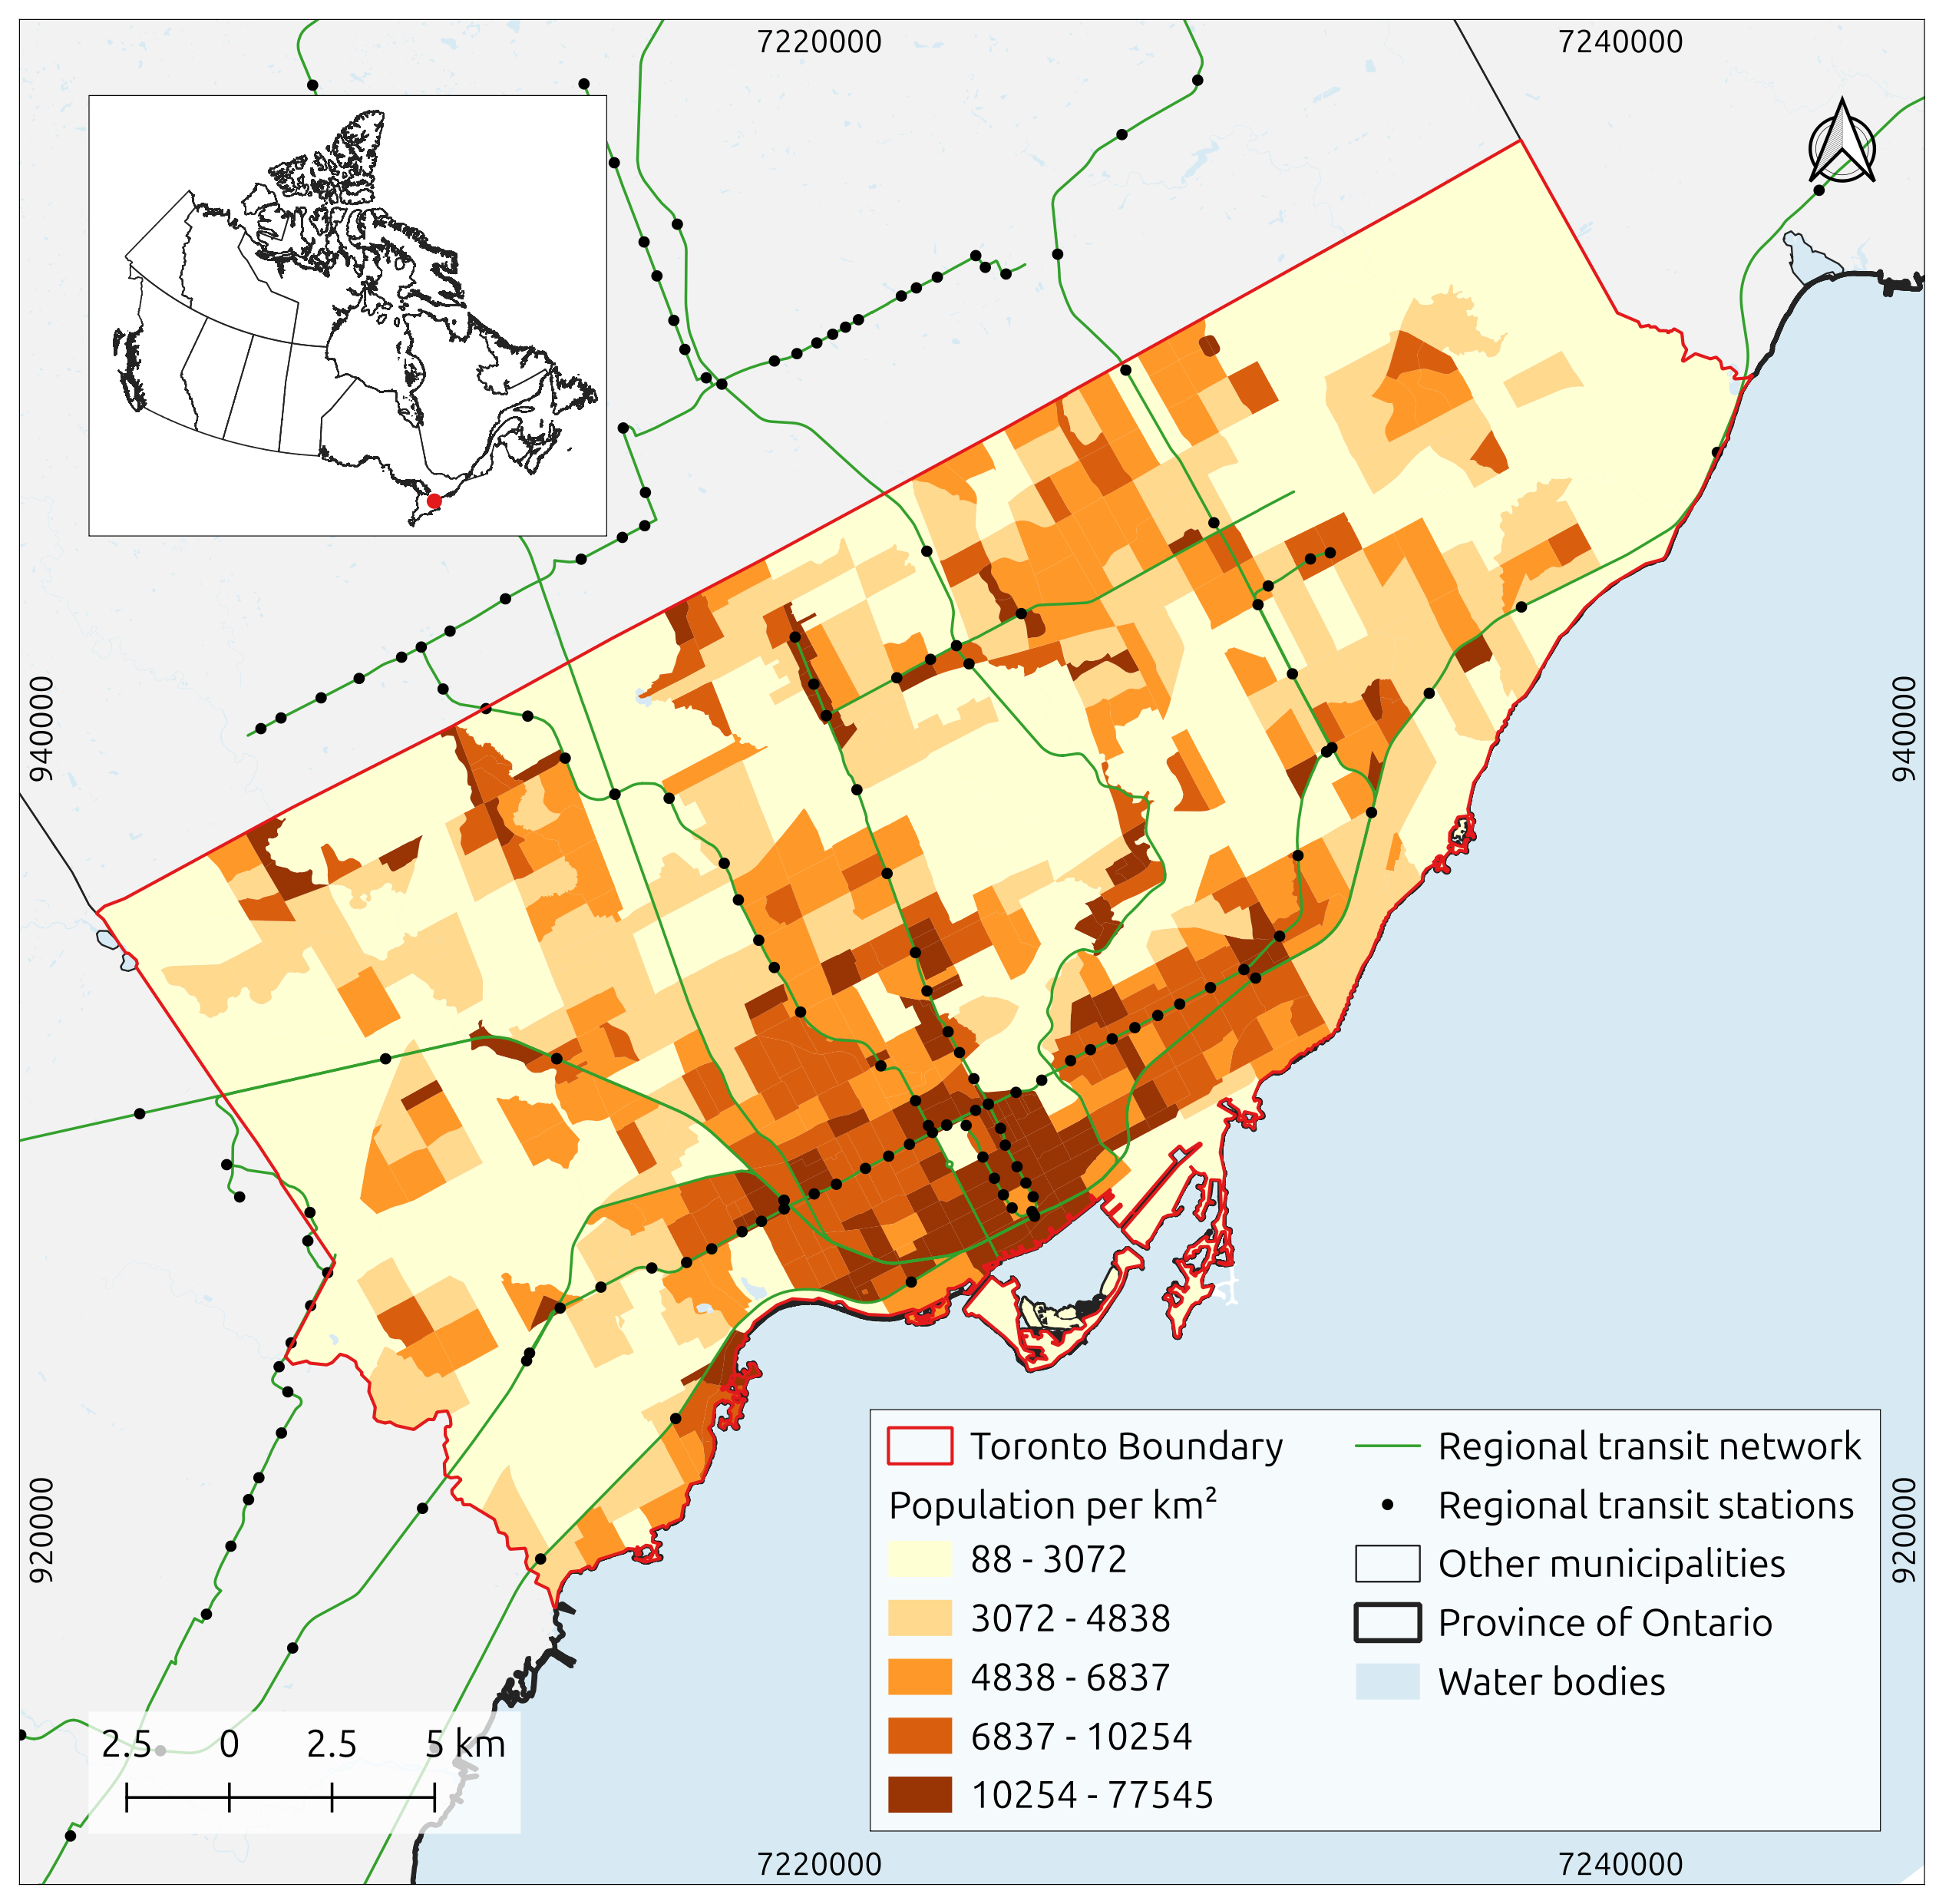
\includegraphics[width=0.8\linewidth]{study_area_map_toronto} \caption{Population density of the City of Toronto (study area).}\label{fig:study-area-map}
\end{figure}

Having defined a study area, we can use one of the \{CommuteCA\} R
Markdown templates to download spatial files using \{cancensus\}. Next,
using \{r5r\}, we can generate routes for the selected transportation
modes and obtain travel-time matrices representing the estimated travel
duration between each origin and destination. These matrices are limited
by the maximum travel times for each transportation mode and Census
Division available in \{CommuteCA\}. Both the methodology for
downloading spatial files and the methodology for generating travel-time
matrices are standardized within the collection of templates.

The \{CommuteCA\} dataset contains 582 of the 585 CTs available in the
study area, with the three missing CTs excluded because they were
subject to Statistics Canada vetting rules. According to our dataset,
the study area has a estimated labour force of around 1,518,405 people
and approximately 1,258,455 job opportunities. According to our
estimates, the majority (61\%) of workers who commute to work in the
study area are car commuters, followed by public transit users (about
27\%), pedestrians (almost 10\%), and cyclists (less than 3\%). Figure
\ref{fig:pop-dens-mode} presents a map of the estimated labour force
population density (per km\textsuperscript{2}) by transportation mode,
created using the \{CommuteCA\} datasets. It can be seen that the
south-central part of the city concentrates a larger active population,
especially walkers, while public transit users and, especially, car
commuters are spread throughout the city.

\begin{figure}
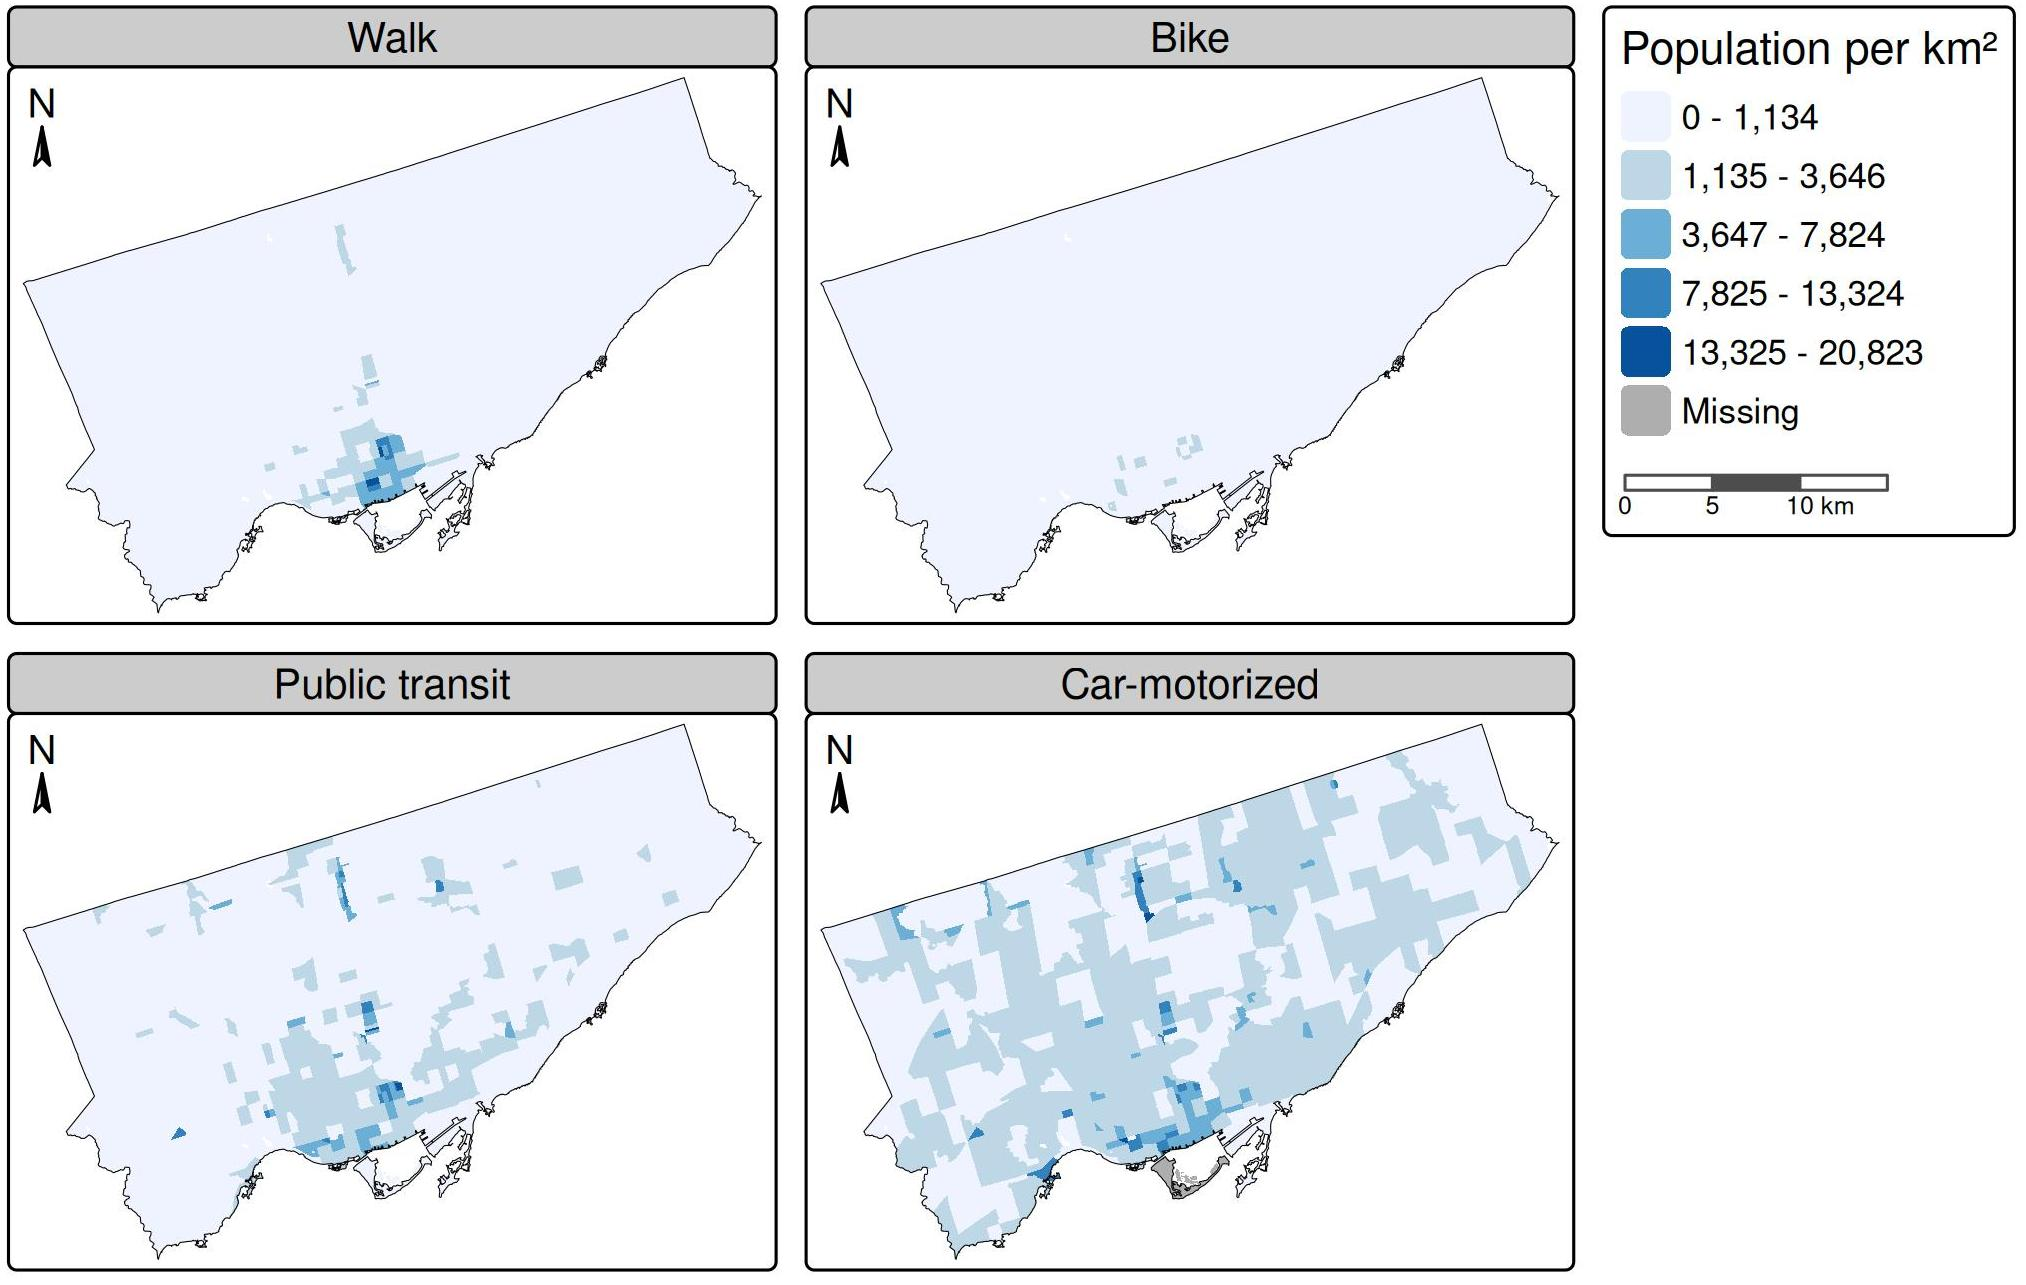
\includegraphics[width=1\linewidth]{density_four_mode_land_use} \caption{Estimated labour force population density by transportation mode.}\label{fig:pop-dens-mode}
\end{figure}

Each transportation mode contains its specific impedance function,
calibrated using only commuters from the City of Toronto. When
calibrated using empirical data, impedance functions illustrate the
distribution of observed commuting travel behaviour across different
travel costs. The analysis of these functions generally reveals a
distance-decay effect, in which greater distances between origins and
destinations lead to lower movement intensity and a lower probability of
observing trips. However, the shape of this distance-decay effect varies
across transportation modes and municipalities, showing differences in
population behaviour when commuting to work.

\begin{table}[H]
\centering\centering
\caption{\label{tab:impedance-table}\label{tab:impedance_functions}Calibrated impedance functions for the City of Toronto.}
\centering
\resizebox{\ifdim\width>\linewidth\linewidth\else\width\fi}{!}{
\fontsize{9}{11}\selectfont
\begin{threeparttable}
\begin{tabular}[t]{llllrr}
\toprule
\multicolumn{1}{c}{\textbf{Census Code}} & \multicolumn{1}{c}{\textbf{Municipality}} & \multicolumn{1}{c}{\textbf{Mode}} & \multicolumn{1}{c}{\textbf{Impedance function}} & \multicolumn{1}{c}{\textbf{Parameter 1*}} & \multicolumn{1}{c}{\textbf{Parameter 2*}}\\
\midrule
 & Toronto & Public transit & Gamma & 3.60068 & 0.07877\\

 & Toronto & Car-motorized & Gamma & 2.32897 & 0.08613\\

 & Toronto & Walk & Gamma & 1.33045 & 0.08492\\

\multirow[t]{-3}{*}[\normalbaselineskip]{\raggedright\arraybackslash 3520} & Toronto & Bike & Log-normal & 2.93888 & 0.64825\\
\bottomrule
\end{tabular}
\begin{tablenotes}
\item \textit{Note: } 
\item For each probability distribution, Parameter 1 and Parameter 2 correspond to their standard defining parameters: the mean and standard deviation (for lognormal and normal), the rate and shape (for gamma), and the power (for exponential).
\end{tablenotes}
\end{threeparttable}}
\end{table}

\begin{figure}

{\centering 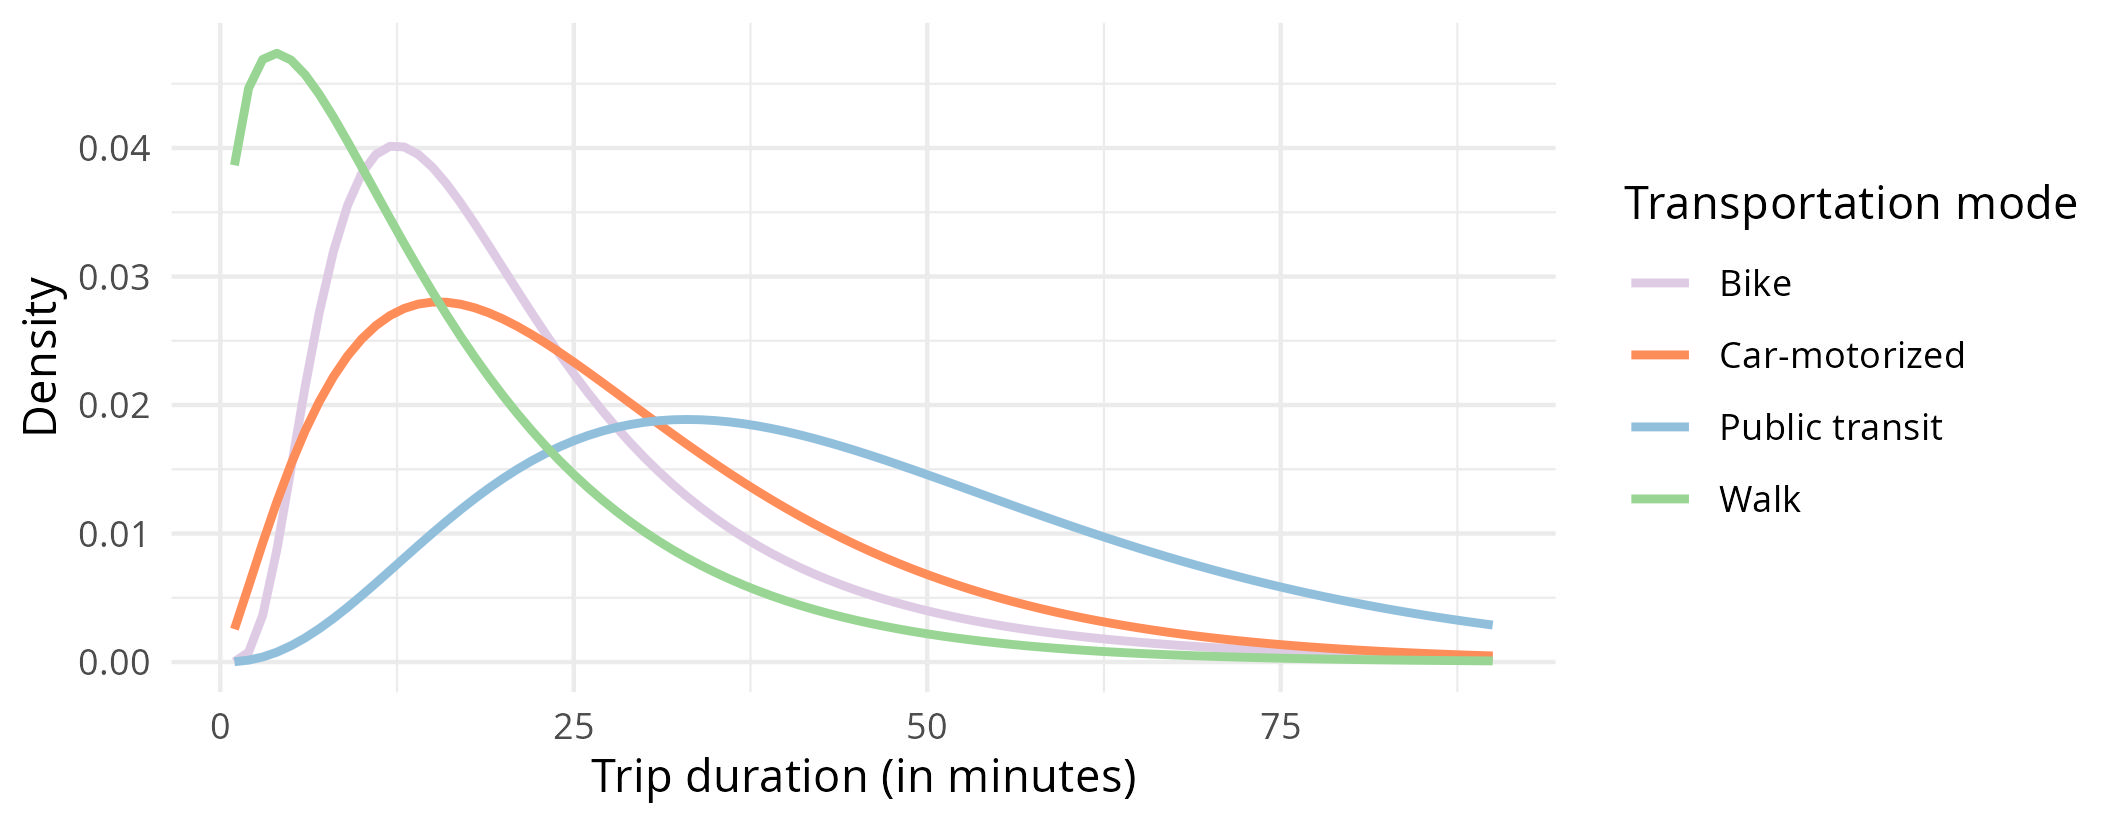
\includegraphics[width=1\linewidth]{mode_impedance_functions} 

}

\caption{Toronto calibrated impedance functions by transportation mode.}\label{fig:mode-functions-fig}
\end{figure}

Table \ref{tab:impedance-table} shows the calibrated impedance functions
for the study area, while Figure \ref{fig:mode-functions-fig} displays
their distributions by transportation mode. Almost all trips are better
represented by gamma distributions, except for bike trips, which are
better represented by a lognormal distribution. In all cases, the
distributions show that at durations close to zero minutes, the trip
density is lower (with a density of zero for public transit and bike
trips). After a few minutes, the density reaches a peak, followed by a
decline toward zero at very high travel durations, indicating a low
probability of observing trips at these travel times.

For walking trips, the probability density peak occurs at around 4
minutes. For cycling trips, the peak occurs at 12 minutes, and a similar
behaviour is observed for car commuters, although the peak occurs at 15
minutes and there is a greater probability of trips continuing to occur
beyond 50 minutes. Finally, public transit users show the longest
commuting durations, with a lower peak density than the other modes and
curves that are more distributed across longer durations. The peak
occurs at 33 minutes. From a transportation planning perspective, these
differences among impedance functions highlight how using a generic
function in accessibility studies can lead to distorted accessibility
indicators, as opportunities may be weighted incorrectly according to
the observed travel behaviour of different populations and
transportation modes.

At this point, the analyst has all the data required to calculate job
accessibility models. Using the \{CommuteCA\} templates, the analyst can
calculate job accessibility and create maps such as those displayed in
Figure \ref{fig:access-fig}.

The maps on the first column show the result of a gravity-based model,
as proposed by Hansen (1959), while the maps on the second column show
the absolute spatial availability and the spatial availability per
person, both proposed by Soukhov et al.
\citetext{\citeyear{soukhov2023a}; \citealp{soukhov2024multimodal}}.
These models differ because the Hansen (1959) model does not consider
competition between people for available opportunities. It has the
advantage of being simple and well established in transportation
analyses. However, its output is not directly interpretable as a number
of accessible jobs, making the indicator more difficult to explain. In
contrast, spatial availability, the measure proposed by
\citet{soukhov2023a} has the advantage of being constrained, meaning
that the model output can be interpreted as the number of jobs
accessible to people in each spatial unit. If we sum the accessibility
values across all spatial units, we obtain the total number of jobs
available in the system. In addition, because it considers competition,
it prevents a single job opportunity from being counted as accessible to
more than one person.

\begin{figure}

{\centering 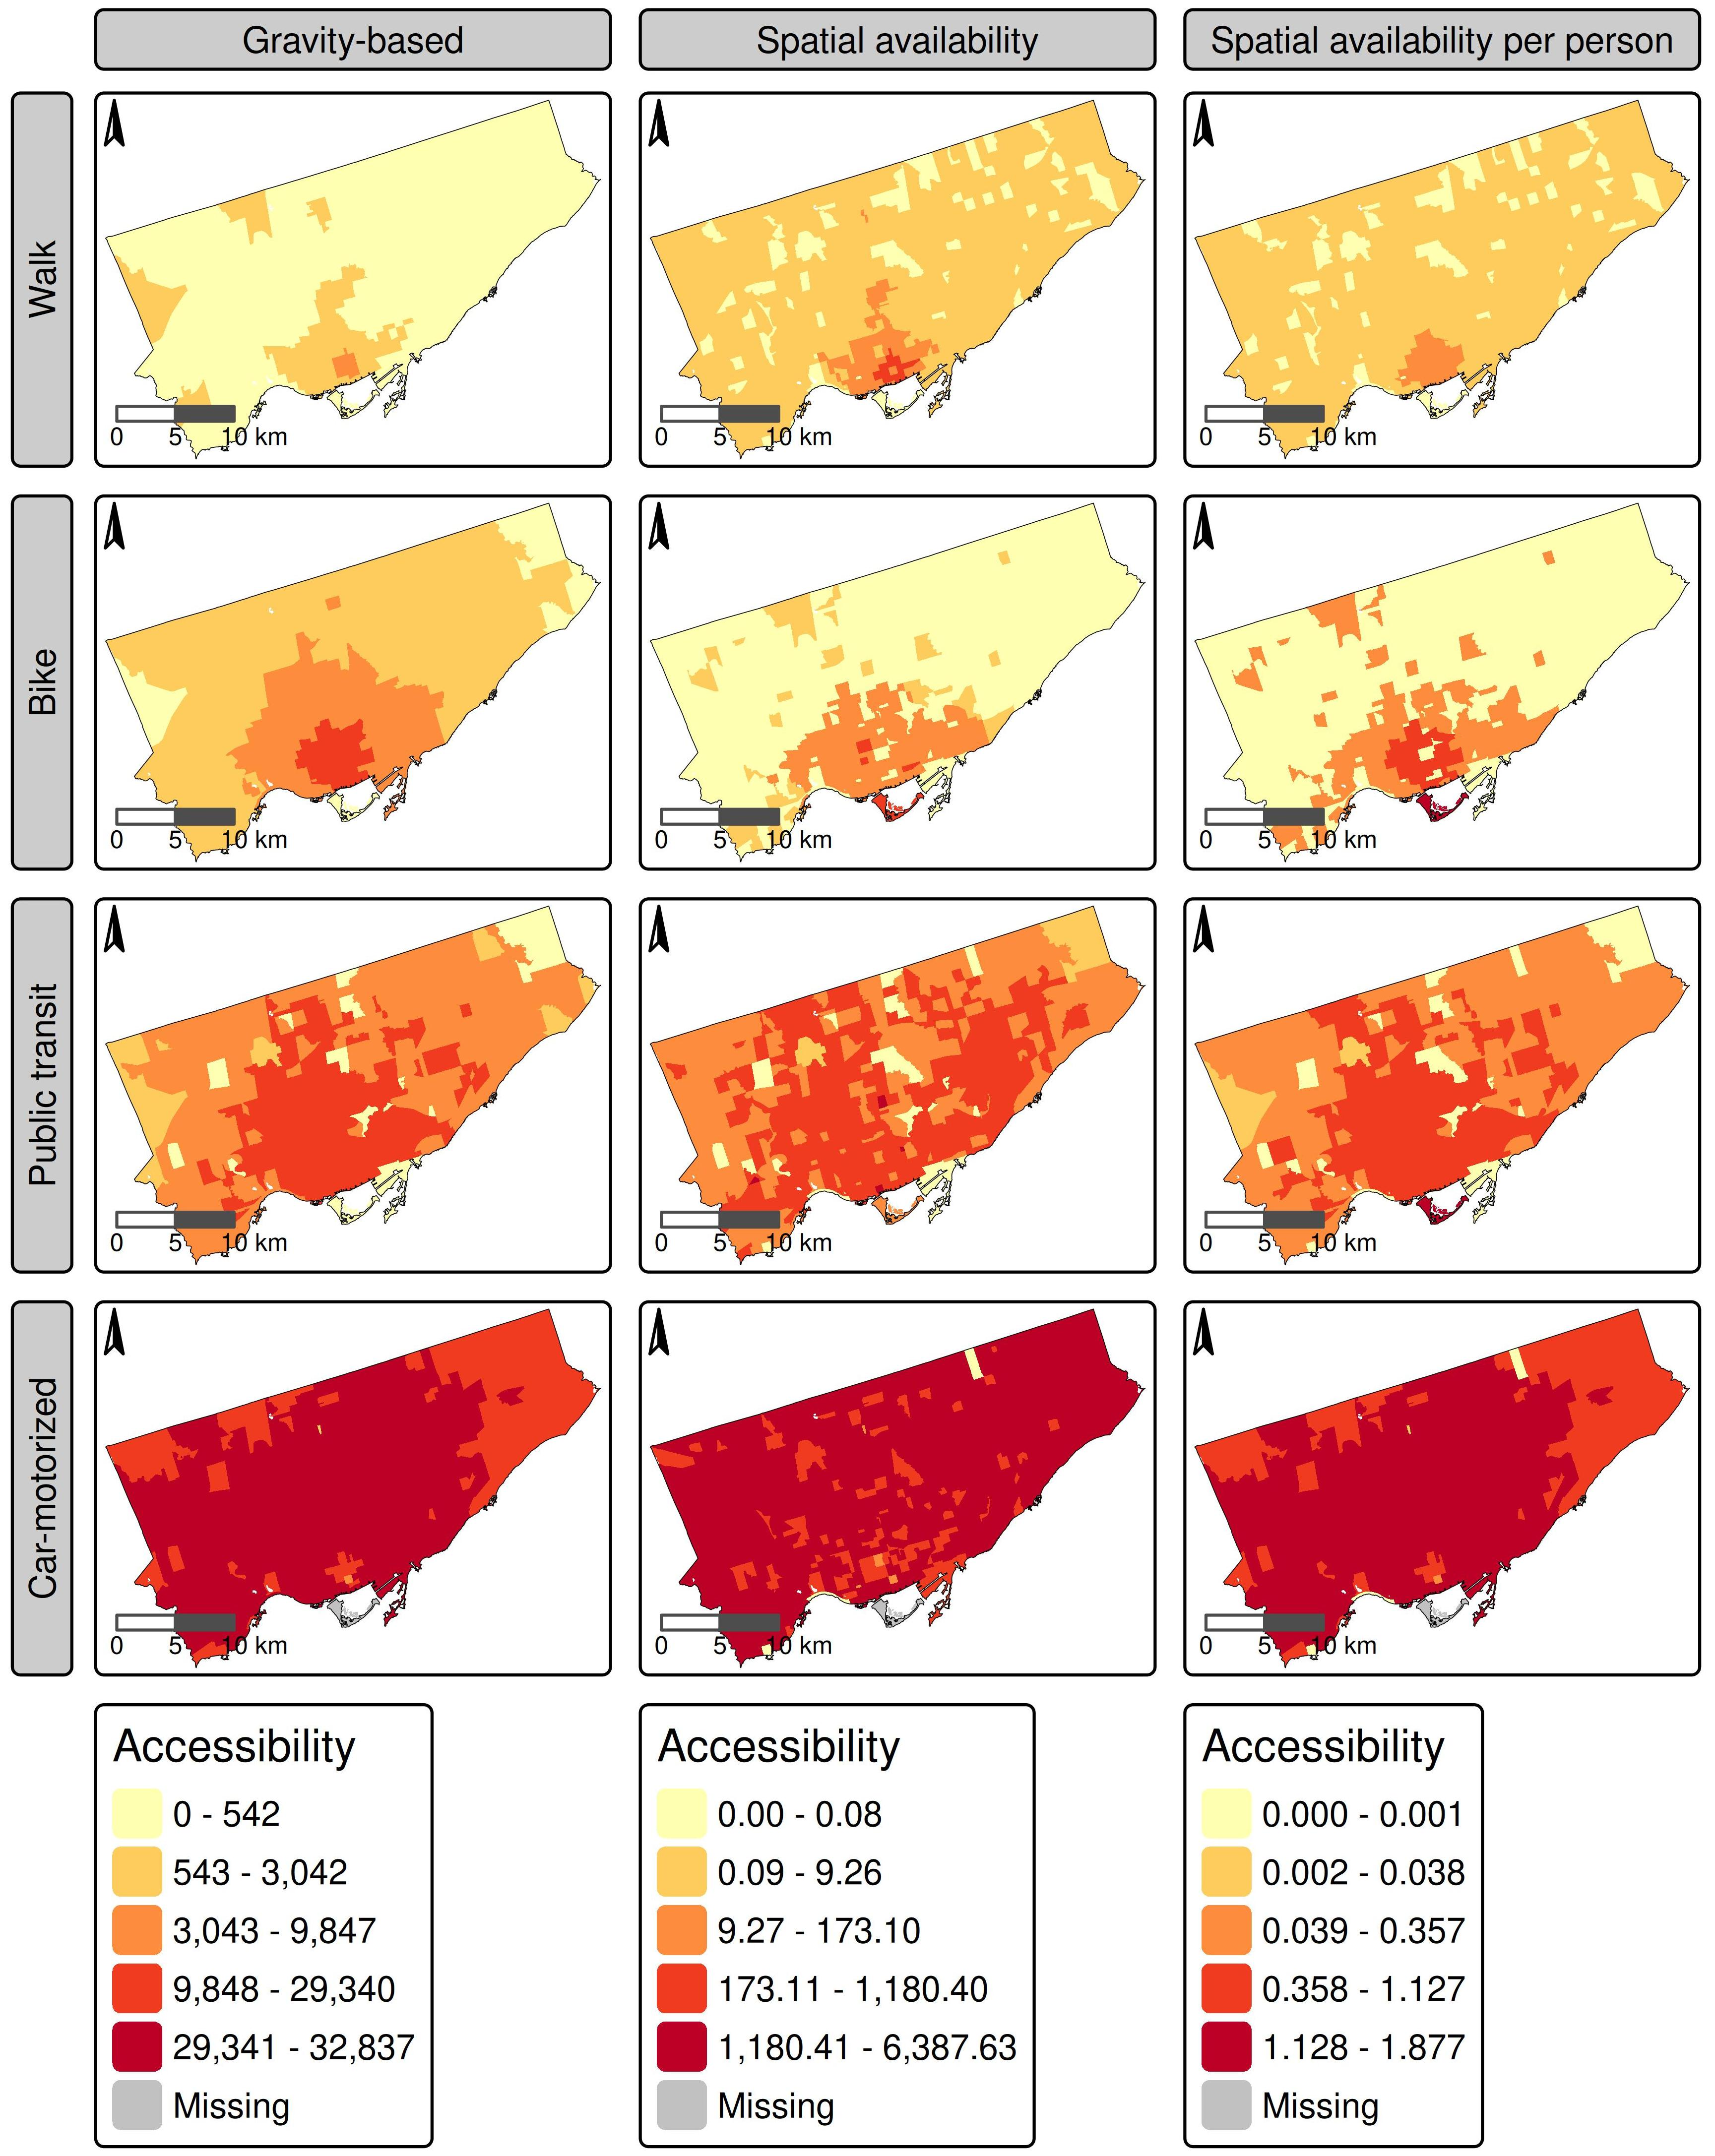
\includegraphics[width=1\linewidth]{four_mode_HT_SA_SApp} 

}

\caption{Job accessibility indicators by transportation mode for the City of Toronto.}\label{fig:access-fig}
\end{figure}

Lastly, the results shown in the third column of Figure
\ref{fig:access-fig} refer to the spatial availability per person, which
refers to the amount of jobs spatially available divided by the number
of people competing for those jobs. This last model is suitable for
situations where the spatial unit (e.g., CTs) does not have a
standardized format, such as regular grids, allowing the comparisons
between areas with different population sizes. As observed for the other
measures, the spatial availability per person shows that, generally, car
commuters can access substantially more jobs than users of other
transportation modes, without large variation across locations within
the study area. In fact, 86\% of the jobs available in the study area
are accessible to people who commute by car, although car commuters
represent 61\% of the study area's labour force (see Figure
\ref{fig:pop-access-shares}). The results for walking and cycling,
however, show that higher levels of accessibility are generally
concentrated around downtown areas. For public transit users, as
expected, higher accessibility is observed in areas with more public
transit infrastructure, such as subway and regional rail lines (see
Figure \ref{fig:study-area-map}).

\begin{figure}

{\centering 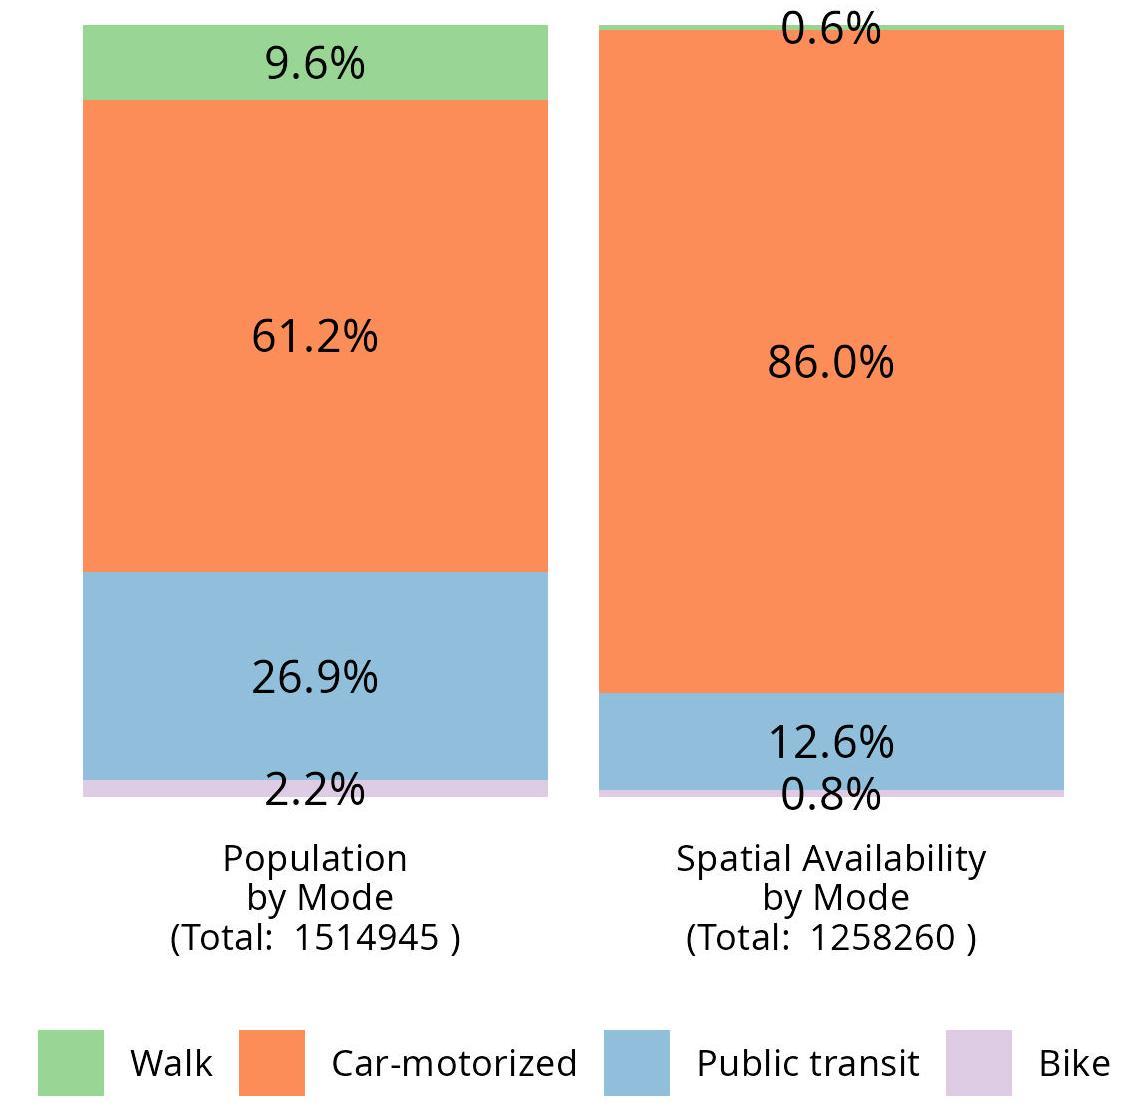
\includegraphics[width=0.5\linewidth]{four_modes_pop_SA_share} 

}

\caption{Share of labour force and jobs spatially availables by transporation mode for the City of Toronto.}\label{fig:pop-access-shares}
\end{figure}

\subsection{Processing 2021 Canadian Census Microdata Files with
\{CommuteCA\}}\label{processing-2021-canadian-census-microdata-files-with-commuteca}

For researchers with access to the restricted microdata files of the
2021 Census of Population, it is also possible to conduct the analyses
shown in our case study at the DA level. Figure \ref{fig:SA-DA-level}
shows the spatial availability measure at the DA level for the City of
Toronto. As shown in the figure, the spatial pattern does not differ
substantially from that observed at the CT level, but for some
applications, a more geographically detailed indicator may be
preferable. In addition, the DA level makes it possible to conduct
analyses for any study area in Canada, which may be relevant for rural
and remote areas where CTs are not available. However, analysis at the
DA level is more likely to have cases excluded during the RDC vetting
process, as we can see from the number of DAs without accessibility
information. This happens because DAs are smaller geographical areas
with lower population sizes when compared to CTs, and are more prone to
failing to meet the population size requirements. As a consequence,
although the high spatial detail of the DA allows for more refined
analysis, these analyses are more likely to be affected by exclusions
during the vetting process.

\begin{figure}

{\centering 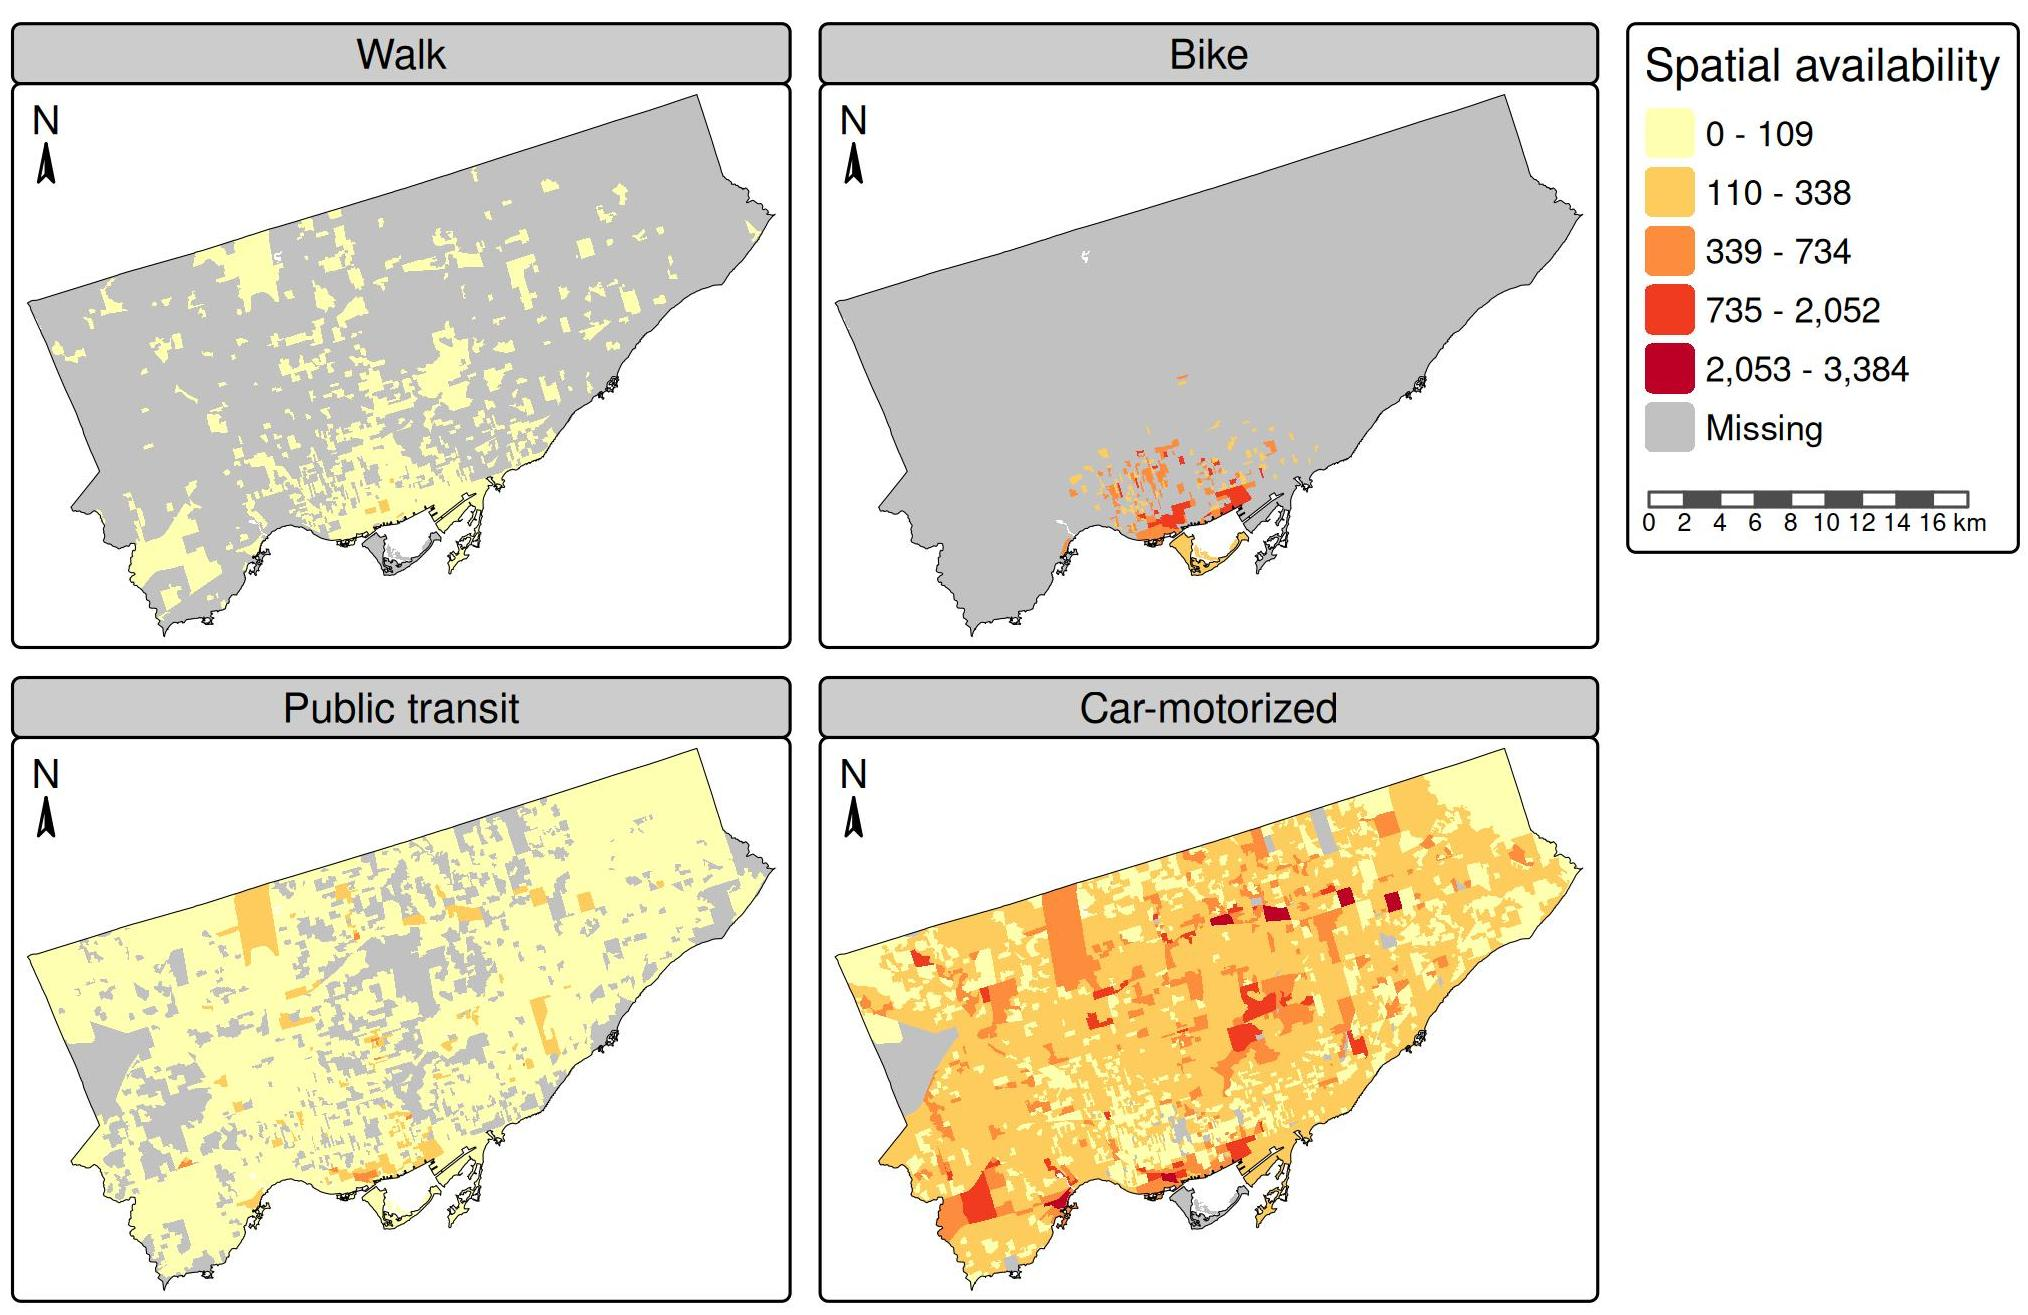
\includegraphics[width=1\linewidth]{SA_four_mode_DA} 

}

\caption{Job spatial availability in Toronto at the Dissemination Area level.}\label{fig:SA-DA-level}
\end{figure}

In addition, \{CommuteCA\} enables researchers to extend the
accessibility analysis by linking accessibility indicators to
socioeconomic and demographic variables. The collection of \texttt{R}
Markdown templates includes instructions for estimating different
regression models to examine how job accessibility is associated with
two employment outcomes: employment status (i.e., the probability of
being employed) and, among those who are unemployed, the probability of
having looked for a job during the four weeks preceding the 2021 Census
interview.

For all \texttt{R} Markdown templates in which census microdata files
are processed, the methodologies include a final code section dedicated
to the Statistics Canada vetting process for RDCs. This section produces
an output formatted according to Statistics Canada rules for releasing
analyses and data derived from census microdata, including comments and
colour-coded spreadsheets to facilitate the verification process by the
RDC analyst while helping protect the confidentiality of census
respondents.

\section{Concluding remarks}\label{concluding-remarks}

Our objective with this article was to introduce \{CommuteCA\}, an ODP
with analysis-ready data and standardized methodologies for job
accessibility analyses in Canada using data from the 2021 Census of
Population. In the form of an \texttt{R} data package, \{CommuteCA\} was
developed after collecting, cleaning, and processing the confidential
microdata files of the most recently released Canadian Census, providing
information on the labour force (classified or not by transportation
mode and education level) and the number of jobs (classified or not by
occupation category) for all Census Metropolitan Areas and Census
Agglomerations in Canada with census tracts. In addition, the package
provides standardized methodologies describing how to conduct
accessibility analyses using the Census microdata files or the already
processed datasets, in addition to customized functions that facilitate
users' analyses.

The package allows users to conduct job accessibility analyses for any
study area in Canada at the Census Dissemination Area level, provided
that the analyst has been granted access to the Census microdata files,
and conduct accessibility analyses for any study area within a Census
Metropolitan Area or Census Agglomeration (where about 84\% of the
Canadian population resides) at the Census Tract level. Similar to other
ODPs, we believe that the value of \{CommuteCA\} lies in its
transparency, accessibility, and ease of use, which facilitates the
addition of complementary datasets in the future.

With \{CommuteCA\}, we aim to contribute to the academic community by
promoting transparent research practices that encourage replication and
innovation in related fields. We believe that this package will serve as
a basis for new research on job accessibility and for the integration of
additional data by authors or the open-source community at large. In
fact, we expect the applications of this package to extend beyond the
range of uses we initially imagined.

\section{Declaration of Conflicting
Interests}\label{declaration-of-conflicting-interests}

The authors declared no potential conflicts of interest with respect to
the research, authorship, and/or publication of this article.

\section{Acknowledgments}\label{acknowledgments}

We would like to especially thank the Research Data Centre analysts at
\emph{to be included} for all their support during the realization of
this study. They guided us on how to work with the confidential
microdata files and how to prepare our outputs in accordance with the
vetting process. This study would not have been possible without their
work.

In addition, we would also like to thank some other \texttt{R} packages
that were essential to the production of \{CommuteCA\}, namely:
\{cancensus\} \citep{cancensus}, \{r5r\} \citep{pereira2021},
\{fitdistrplus\} \citep{delignette2015fitdistrplus}, \{tmap\}
\citep{tmap}, \{sf\} \citep{sf}, and packages within the \{tidyverse\}
initiative \citep{tidyverse} - especially \{ggplot2\} \citep{ggplot2},
\{dplyr\} \citep{dplyr}, and \{tidyr\} \citep{tidyr}.

\section{Funding}\label{funding}

The work has been supported by funding from the \emph{description about
the funding source after the review process}.

\section{ORCID}\label{orcid}

\begin{itemize}
\tightlist
\item
  Anon1 - \url{https://orcid.org/}
\item
  Anon2 - \url{https://orcid.org/}
\end{itemize}

\section{Data availability statement}\label{data-availability-statement}

The \{CommuteCA\} \texttt{R} data package can be found and installed on
\href{https://github.com/}{Github}.

For review purposes, the package is currently available as a tar.gz file
that can be installed by R. The file can be obtained from this anonymous
location: \textless{}\emph{to be included}\textgreater{}

\bibliographystyle{sageh}
\bibliography{bibfile.bib}


\end{document}
